\chapter{Serverless computing}

\section{Origins}

The growth of cloud computing significantly influenced the way how server management and server application development are perceived. Around fifteen years ago, most of the companies were entirely responsible for managing their software, altogether with the hardware and infrastructure it was running on \cite{RobertsChapin2017}. Around that time, first services capable of outsourcing some part of infrastructure overhead emerged, which started the idea of cloud computing.

Amazon Web Services was one of the first service providers that enabled companies to rent computing capacity by announcing the launch of Elastic Compute Cloud (EC2) in August 2006. It was the first Infrastructure as a Service (IaaS) product on the market that allowed companies to run their server applications on Amazon's machines that are billed per usage time and are available within minutes from requesting new resources.

Leveraging such a service model brings a handful of benefits. It reduces the labour cost by outsourcing hardware management to the provider and infrastructure cost by paying based on actual usage of services. Furthermore, it enables companies to scale the number and type of servers in correlation with the traffic and demand for processing. Finally, it encourages testing new solutions developed by companies by decreasing the lead time, by making the required infrastructure available within minutes instead of months, utilising favourable billing flexibility.

The cost of IaaS solutions is profitable to providers, because of technical improvements done in terms of hardware virtualization and the economy of scale on which they operate. Shortly after other vendors such as Microsoft, Google and DigitalOcean embraced the notion of public cloud by providing services and resources from their own data centers. At the same time, tools like Open Stack enabled companies to use hardware from their own data centers in the same way, forming the idea of private cloud.

The next step in the cloud evolution is Platform as a Service (PaaS). As a layer on top of IaaS, it adds operating system to the outsourced infrastructure stack enabling to deploy the application code directly. In that model, the platform takes responsibility for managing the operating system as well as monitoring and running the application. Google App Engine, AWS Elastic Beanstalk and Heroku platform can be distinguished as most popular PaaS solutions, while one of the most frequently mentioned self-hosted variant is Cloud Foundry.

The growth of containerisation technologies introduced another type of service called Container as a Service. Technologies like Docker allowed developers and system administrators to deliberate more clearly on the application requirements and separate it from the operating system. Solutions such as Marathon running on top of Mesos and Kubernetes introduced a possibility to manage and orchestrate containers on self-hosted machines. The services provided by cloud vendors include for example Google's Compute Engine or Amazon's Elastic Container Service (ECS) or AWS Fargate. With the growing popularity of Kubernetes, dedicated services leveraging that platform such as Amazon Elastic Kubernetes Service (EKS) and Google Kubernetes Engine (GKE) emerged.

Each of the described services are next generations of infrastructure outsourcing, which raise the level of abstraction from the development perspective and hand off more and more responsibility related to infrastructure management to the cloud vendor. Despite the fact, for each of the mentioned services the smallest unit of processing is some sort of server application or running application process in the virtual machine or within the container.

Serverless is considered as a next step in the cloud computing progression. The term serverless was one of the first used by Ken Fromm in his paper \cite{KenFromm}. It describes the notion of architecture migration from monolithic applications running on servers into distributed systems that consist of multiple components, processes and data stores with the goal to perform various tasks and process numerous flows. The serverless architecture enables developers to make a mindshift accordingly. Computing resources can be used as services, which makes it possible to shift thinking from the servers level to the tasks level, taking away the complexity of infrastructure management. The servers are still used underneath, but developers don't need to worry about managing them any longer.

Such an architecture model was leveraged firstly by mobile applications built on top of hosted database solutions such as Parse (later acquired by Facebook) and Firebase around 2012 (obtained by Google). Nonetheless, the most significant event shaping the serverless architecture was the announcement of AWS Lambda in 2014, altogether with the introduction of API Gateway in 2015. By the middle of 2016, major cloud vendors such as Microsoft and Google embraced the serverless architecture approach and started offering their services for developing serverless applications.

\section{Defining serverless}

Despite the fact that the idea of serverless computing emerged about a decade ago, it has been already widely adopted by leading cloud providers. Currently it covers a range of technologies, components and cloud services. Nevertheless, there is no clear and concise view on what ''serverless'' is. Various vendors, organisations and research groups tried to define what the serverless term means for them.

Cloud Native Computing Foundation of the organization working towards standardisation of numerous cloud-related technologies and components. It maintains a sustainable ecosystem for cloud native software by bringing together and collaborating with various members of the cloud community. According to ''CNCF Serverless Whitepaper'' \cite{CNCFServerless}.

\begin{quotation}
Serverless computing refers to the concept of building and running applications that do not require server management. It describes a finer-grained deployment model where applications, bundled as one or more functions, are uploaded to a platform and then executed, scaled, and billed in response to the exact demand needed at the moment.
\end{quotation}

Another definition considering the serverless service capabilities can be found in a booklet made by Mike Roberts and John Chapin titled ''What is Serverless?'' \cite{RobertsChapin2017}.

\begin{quotation}
\noindent A Serverless service:
\begin{itemize}
    \item Does not require managing a long-lived host or application instance
    \item Self auto-scales and auto-provisions, dependent on load
    \item Has costs that are based on precise usage, up from and down to zero usage
    \item Has performance capabilities defined in terms other than host size/count
    \item Has implicit high availability
\end{itemize}
\end{quotation}

The cited definitions contain insightful information about features of serverless architecture and capabilities of its components. These can be summarized as follows:

\begin{itemize}
    \item Serverless architecture defines the new model of developing and executing workloads. The application consists of multiple serverless components configured together to run the business logic within the application code, designed to be executed in a serverless environment.
    \item It does not require to maintain, provision and monitor servers and applications. Serverless does not mean that there are no servers - the overhead of managing them is handed off to the cloud provider.
    \item Deployment model is more granular. Having the application built from multiple components configured to work together, the deployment can update only selected ones.
    \item Platform is responsible for provisioning and executing the applications. With a large resource pool maintained by cloud provider and the possibility to quickly allocate it, the solution can be scaled automatically to the current load requirement almost instantly.
    \item The cost is proportional to the resource usage. Each of the components involved in performing the computation is billed granularly, with an accuracy to hundreds of milliseconds or number of executed operations, with no cost when being idle. Executing hundred operations in parallel will cost the same amount of money as running that workload sequentially.
    \item The performance is not related to the host size. Some of the cloud providers enable customers to choose how much memory and CPU can be allocated for the environment. Nevertheless, the configuration is abstracted from the capabilities of the underlying machine that is used as an application execution environment.
    \item The serverless components are built with high-availability and fault-tolerance in mind. Despite the fact that developers are no longer concerned with servers, the underlying vendor's machines can still fail. When using serverless services we expect that cloud vendors will provide transparent high availability for its services. Although, as developers it may be necessary to handle some errors and failure occurrences properly.
\end{itemize}

\section{Serverless components}

When considering the serverless architecture we refer to a range of technologies provided by cloud platforms. Two different areas can be distinguished, defining two distinctive components:

\begin{itemize}
    \item \textbf{Backend as a Service} refers to third-party services or generic components capable of replacing some part of a server side application, that has been previously developed internally or self-provisioned. It exposes an API which allows for integrating the component with the rest of the application.
    \item \textbf{Function as a Service} is an event-driven execution environment for running application code within stateless and ephemeral containers with strictly limited execution time.
\end{itemize}

Aforementioned components used simultaneously enable developers to build fully-fledged solutions utilising serverless architecture and are offered together within a single cloud platform.

Even though presented areas serve different roles, they share common features and capabilities. These could be listed as follows:

\begin{itemize}
    \item Require no resource management and are entirely provisioned by cloud provider
    \item Billing is proportional to actual usage
    \item Utilise the event-driven model for processing
    \item Underlying platform ensures automatic horizontal scaling, high availability and fault tolerance
\end{itemize}

\subsection{Backend as a Service}

The concept of Backend as a Service (BaaS) gathers various domain-generic, repeatable application components capable of replacing some part of application logic or providing some functionality. They can be accessed and integrated into developed applications through API defined by its provider.

Taking into consideration most popular requirements of various applications, the majority of them need to store and manage the data. Depending on the requirements the information should be stored in a structural way in databases or can be stored regardless of their shape in file storage service. For teams developing mobile or web applications it is convenient to rely on some third-party service to store and access the data directly from the application. Services like Google's Firebase meet such requirements and give access to the database entirely managed by a cloud vendor. Depending on the complexity of developed product it may be required to incorporate some more advanced components to process required tasks or flows reflecting the business logic of application. Mechanism serving as notification services, exposing some publish-subscribe capabilities for defined events could be applicable in that case. It is essential to notice that such components are replacing previously self-hosted components such as databases or other data stores, message-brokers or other services responsible for processing data streams incoming from various sources.

Looking closer from the application logic point of view, there are also repeatable functionalities implementations that can be extracted and reused across multiple developed applications. Most of the products will require some features enabling users to manage their identity and associated permissions. Most of the time, the capabilities will be not only limited to registering and logging users, but it will also include integrations with other services as identity providers. Managing and sending emails can be considered as another functionality that can be extracted into separate component from the code perspective and reused in other applications. Products such as Auth0 (serving as fully featured authorization and user management service) or Mailgun (capable of managing and processing emails) makes it possible to replace entirely the repeatable part of business logic.

% TODO:rb update chapter reference
Specific components and services that can be classified as Backend as a Services will be covered in more details in chapter ... when analysing services provided by leading cloud vendors. All of the mentioned components enable developers to create fully fledged applications and services similar to the solutions built using self-hosted component equivalents. The difference is that mentioned components are characterized by capabilities of the serverless architecture. They are provided by cloud vendors, who take responsibility for managing, provisioning and scaling them depending on the demand. Moreover, the possibility to replace the repeatable application features by utilising third-party services enables developers to iterate faster and shorten the lead time.

\subsection{Function as a Service}

The second area refers to Function as a Service (FaaS) that serves as an environment for executing application code. It introduces a new architectural approach in terms of developing, structuring and deploying the application logic, which is oriented towards individual tasks and operations.

Mike Roberts briefly described the idea of FaaS \cite{MartinFowlerServerless} based on the definition of AWS Lambda \cite{AWSLambda}, which is currently one of the most commonly used implementation of a Function as a Service platform. Based on his summary several main features of FaaS can be highlighted:

\begin{itemize}
    \item The main idea of FaaS is to run application code without managing servers and application processes. It is a common feature with other approaches like CaaS or PaaS, where the responsibility for managing applications is placed on the cloud vendor. However, the key difference with FaaS is the fact that the function execution time is strictly limited in contrast to long-lived processes existing in aforementioned services.
    \item The functions are invoked and executed on the underlying platform in response to specific events occurring or incoming into the system. Based on that cloud provider handles resource allocation and runs the function code in an ephemeral container, created based on runtime needs. These are destroyed shortly after the event is processed by the application logic in the function. Together with limited execution time it is a significant architectural restriction for the FaaS model.
    \item Given the fine-grained execution model, horizontal scaling can be easily and automatically handled by the cloud provider. When there is an increased traffic in the system, the platform responsible for executing functions allocates resources to create and run more functions, which will be capable of processing the increased traffic. An analogous situation takes place when there is no traffic, therefore there is no need to allocate resources for running functions code.
    \item As a consequence of greater granularity of application code and managing the function execution by cloud provider, the deployment process differs from the traditional system. Each function can be independently packed and uploaded to the FaaS platform, which takes responsibility for executing it.
    \item Most of the cloud platforms do not require to use neither predefined framework nor programming languages. Although cloud providers define the list of environments and languages that are supported by the platform, any process that is bundled into the artifact and can be executed from it is capable of processing the incoming event.
\end{itemize}

Selected aspects of Function as a Service architecture are covered in more details based on ''CNCF Serverless'' whitepaper \cite{CNCFServerless} in the following sections.

\subsubsection*{Function lifecycle}

Before analyzing the execution model in more details, it is important to examine the deployment process accompanying the development of a function. Alongside with providing the function code, the developer is responsible for specifying one or more events upon which function will be triggered. Additionally, metadata defining for example the function version, environmental variables, execution role and other configuration parameters can be defined. The function and specification prepared in that way is uploaded to the cloud provider and processed by a dedicated builder entity, resulting with a function artifact (depending on the cloud platform and selected runtime it can be a binary file, container image or a package). Next, it is deployed on a cluster managed by a FaaS controller responsible for provisioning, controlling and monitoring function instances based on incoming events.

\begin{figure}[h]
    \centering
    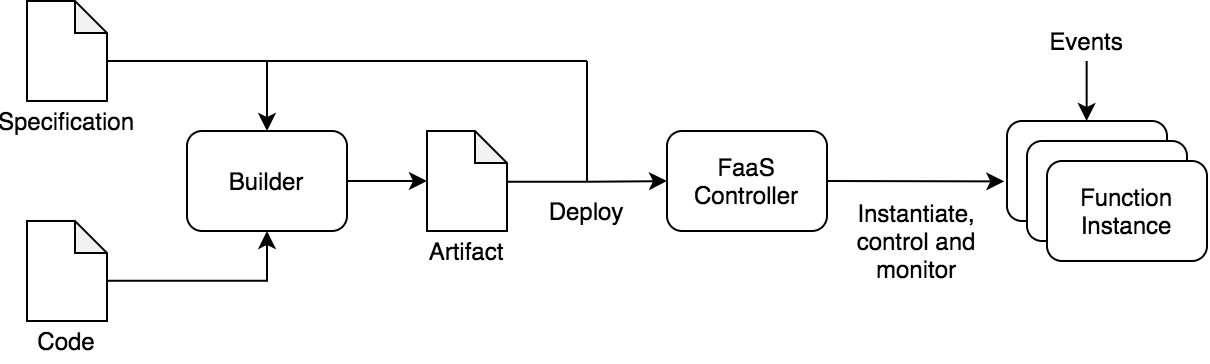
\includegraphics[width=0.8\textwidth]{assets/02-serverless/ServerlessDeployment.png}
    \caption{Function deployment and invocation process}
    \label{fig:cloudguru-architecture-diagram}
\end{figure}

Furthermore, the serverless platform may provide additional actions related to function management such as executing, publishing, updating and deleting the function or its metadata. Also, a particular version of the function can be labeled or aliased, which can come in handy when operating the serverless system on a larger scale. Logs and statistics are gathered alongside function execution.

The function is executed in an event-driven model and within strictly limited duration. The whole process begins when an event triggering a particular function is dispatched. It is detected and registered by an underlying serverless platform. The controller responsible for managing function execution looks for functions associated with incoming events, gets its code and configuration and allocates an adequate amount of resources from the managed resource pool. The new execution environment is created inside a lightweight, ephemeral container and language runtime for the function is bootstrapped. When it's ready, the triggering event is redirected and processed by the application logic contained in the function code.

The results of computing are sent back to the event dispatcher. Other, newly created events can be dispatched during function execution. The computing duration is limited by the majority of service providers up to a few minutes, after that the computation is completed with timeout. At the end the lightweight container containing the execution environment is destroyed.

Most of the providers delay the container deletion for longer than a couple of minutes due to optimisation related with reusing the same container instance when the next event occurs in the system. Reusing an already initialised execution environment is called a ''warm start'' and allows to reduce the startup latency related to resource allocation and runtime preparation. The opposite situation takes place when the new container instance needs to be initialised and the host process needs to be created. Most of the time it requires additional time impacting the request processing duration - it is called ''cold start''.

\begin{figure}[h]
    \centering
    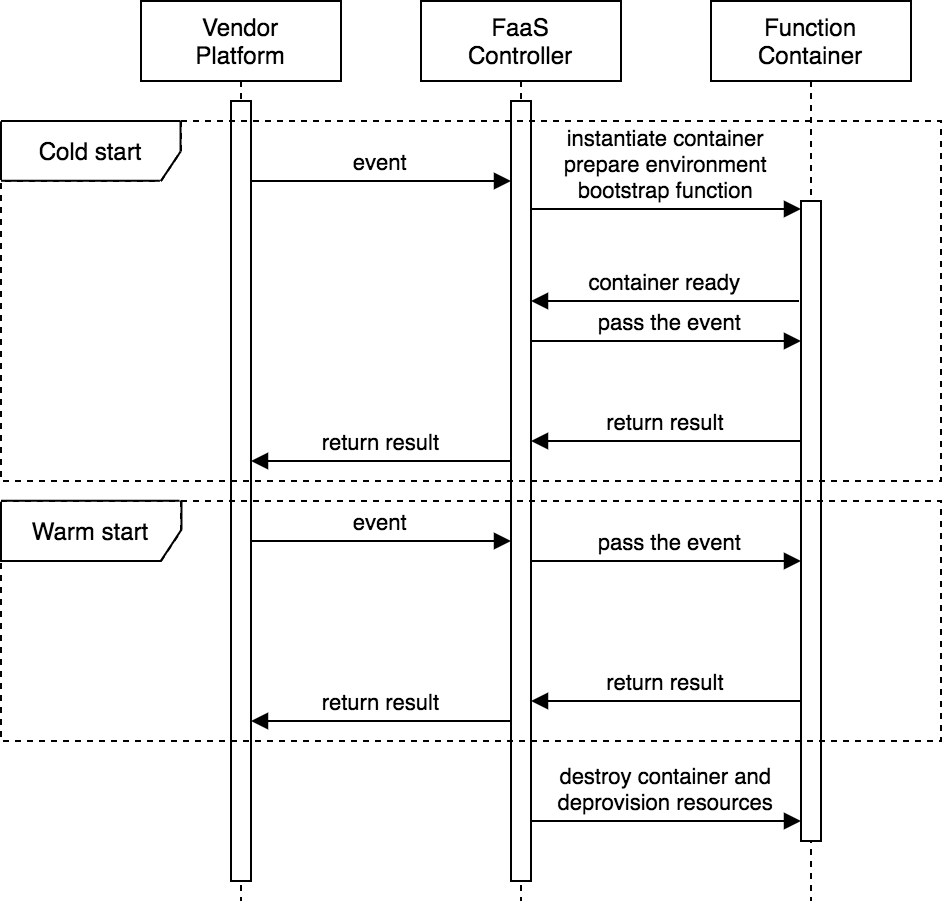
\includegraphics[width=0.7\textwidth]{assets/02-serverless/ServerlessExecution.png}
    \caption{Function execution process considering ''cold start'' and ''warm start''}
    \label{fig:cloudguru-architecture-diagram}
\end{figure}


\subsubsection*{Function environment}

The characteristic of the function environment has been already drafted during description of the function lifecycle. Due to improvements in the software virtualisation area, cloud vendors can benefit from efficient and elastic management of large resource pools. It enables vendors to allocate efficiently lightweight and ephemeral containers, serving as an execution environment. Each of them is initialised to execute code of one of the functions at a time and it is destroyed shortly after, releasing the resources to the common pool. Even though containers can be reused for the optimisation purposes when handling subsequent events occuring in the system, it is not guaranteed by the serverless platform and should not be taken for granted by developers, that some data could be preserved for subsequent invocation.

Such an architecture leveraging stateless containers allows for automatic horizontal scaling. When multiple concurrent events occur within the system, the platform is capable of creating a separate container to process each of them independently. In order to handle spikes of traffic effectively, quick provisioning of the containers and reducing their startup latency is required and it is a purpose many research works and improvements made by both researchers and cloud vendors

As mentioned before, ephemeral containers are dismissed shortly after the execution alongside with their internal state. For some types of computing it would be desirable to preserve that state. To address that issue, external components need to be introduced to persist the data. Nevertheless, it introduces the need to communicate with some external service and it is often associated with additional delays resulting from the communication overhead.

\subsubsection*{Function invocation}

The serverless architecture utilises an event-driven processing model. The developer's task is to define configuration that maps events coming to the system with appropriate functions. Each of dispatched events can trigger one or more functions as well as each function can be invoked by one or more predefined events - there is a many-to-many association between function and event sources. The mapping can also refer to a particular version of the function or alias, which can greatly simplify the deployment process by replacing the function code for a given alias without modifying the configuration.

Various data sources can be divided into several categories among which we can distinguish:

\begin{itemize}
    \item Endpoint Services - Most of the time associated with API Gateway components, which introduces mapping between request coming from APIs, such as REST or Websocket and associate them with corresponding functions
    \item Storage Services - Category includes numerous BaaS components provided by a cloud vendor like databases, file storage or cache services. Events can be emitted based on operations performed on the data such as creation, deletion or modification of it.
    \item Messaging Services - Services providing mechanisms for data streaming, message brokers or various services sending notifications.
    \item Scheduled events - That category include services capable of emitting events periodically at a given time or at a selected interval
\end{itemize}

Based on the use case, several invocation types can be differentiated:

\begin{itemize}
    \item Synchronous Request - Includes cases when the client sends a request and waits for the response. It is used most frequently for HTTP requests.
    \item Asynchronous Message Queue Requests - Refers to events emitted from various data sources when messages are published to some exchange that later distributes it to other subscribers. Messages are delivered exactly once without strict ordering.
    \item Event Streams - Are based on streams of messages, logs or files. Sequence of record is most of the time partitioned into several shards.
    \item Batch Jobs - Refers to jobs that can be splitted into smaller tasks and processed in parallel by multiple functions. The entire process is completed when all subsequent tasks are finished.
\end{itemize}

\section{Benefits and challenges}

The emergence of serverless architecture has met with great interest from various companies that noticed numerous advantages of utilising the serverless approach. In addition to the promise of a significant cost reduction there are many others benefits related with development and operational side that made serverless architecture desirable. 

Nevertheless, serverless architecture also has many disadvantages inherently connected with it's nature. Some of them has been addressed by various cloud vendors working towards improving their services and mitigating the problems. Despite the fact that many companies adapted it the technology is not fully mature yet. There are many research underway in various areas by both researchers and cloud vendors.

Among the many reports and articles \cite{MartinFowlerServerless} \cite{BerkeleyServerless}, you can find listings of benefits and challenges assigned to the serverless architecture. These has been categorized and listed below.

\subsection{Benefits}

\subsubsection*{Operational cost reduction}

Serverless is another step in process of infrastructural outsourcing that started a few years ago when idea of Infrastructure as a Service emerged. 
The responsibility for managing and operating systems and other components it transfered to cloud provider, which is a common feature with IaaS and PaaS solutions.
What's different is the fact that serverless architecture introduces various BaaS elements that can replace selected parts of the application and bring significant reduction of development cost.
This brings serverless architecture closer to its promise in which developers can focus on application logic while the responsibility of managing resources and delivering required services is moved on to the underlying cloud platform.

\subsubsection*{Autoscaling with proportional cost}

Another key feature of serverless architecture is automatic and elastic horizontal scaling handled entirely by provider. 
It is also directly connected with the cost that is proportional to amount of resources needed to handle the demand for processing. 
With granular billing plan for most of the components it can bring significant cost reduction especially for services characterized by inconsistent or occasional traffic.
The load is handled autoamtically by cloud platform which manage resource allocation based on demand and reduce amount of working components when system utilization decreases. 
It mitigates also problems of under-provisioning (when the system capacity was optimised for average traffic that could not be sufficient for heavier load) and over-provisioning (when the capacity of the system was prepared to work efficienly when traffic reached the top, but for modest load the available capacity was not entirely utilised).

% optimization - root of cost savings - with pay as you go and granular payment model each optimisation brings instant cost savings

\subsubsection*{Development improvements}

The application development process can be accelerated by leveraging numeroues BaaS services. Some of the well-developed and tested components can be integrated with the application logic replacing self developed modules. 
It can significantly decrease the initial development process from basic idea to working prototype build from handful of functions and components configured to interact with each other building the business logic. 
Furthermore, deployment of serverless application is also more convenient. Each of the function is separatelly packed and deployed with metadata to the cloud platform that takes responsibility for the rest. There is no need for adjusting and managing configuration or software on the host machines.

\subsubsection*{Reduced time to market}

Utilising the benefits of easier infrastructure outsourcing, reducing operational management and accelerating development speed, serverless architecture appears to be a concept desired by many product owners. 

In the era of lean and agile processes it can be used to quickly test and develop new features for existing applications... %  TOOD

% It can be leveraged to launching new features quickly.
% ... lean architecture -> towards continuous deployment

\subsubsection*{Greener computing}

% ---

\subsection{Challenges}

% \subsubsection*{Vendor dependence}

% loss of control

% \begin{itemize}
%     \item by using BaaS / cloud platform - giving up control of system
%     \item serverless systems can also have downtime - provider's issues
%     \item unexpected limits for particular services
%     \item changes in functionalities / forced API changes
% \end{itemize}

% vendor lock-in

% multitenancy problem

% \begin{itemize}
%     \item multiple instances of different customers running on the same machine - efficient for customer (economy of scale)
%     \item improvements in virtualization - for customer may seem that we're alone in the system - some times problems with security (see data of others), robustness (error for one customer propagates to other), performance (one customer takes most of the resources)
% \end{itemize}

% security

% \begin{itemize}
%     \item using BaaS directly from mobile platforms - loss of protection from server side
%     \item each function + metadata = resources security policy - give lowest possible access, how to manage them properly across whole organisation
% \end{itemize}

% \subsubsection*{Architecture limitations}

% start up latency - cold start

% stateless - need external storage to persist data

% \subsubsection*{Development challenges}

% testing

% debugging

% complexity of development

% \subsubsection*{Operational challenges}

% deployment

% monitoring

\noindent\makebox[\linewidth]{\rule{\paperwidth}{0.4pt}}

Based on
\cite{MartinFowlerServerless}
\cite{RobertsChapin2017}
\cite{BerkeleyServerless}
\cite{BerkeleyServerlessComputing}

The architectural design that makes functions autoscalalble makes it also not suitable for some types of workloads

Use cases

- leveraging lambda for independent tasks that can be easily paralelized
- orchestration function - calling other services
- function composition - functions chained together to manipulate some state - login workflow

- simple workloads of independent tasks - parallel tasks embedde in lambda functions
- stateful tasks requiring low latency may be not suitable for that

\subsection{Benefits} 

\subsubsection*{Auto scaling with proportional cost}

- horizontal scaling is entirely automatic, elastic and managed by the provider
- you pay for execution duration of functions instead of allocated resources (down to 100ms or even 1ms in case of AWS Lambda)
- occasional requests - no need to keep server idle most of the time, encourage companies to try out new features - extremely small operation cost with relatively small workloads
- inconsistent traffic - autoscaling with paying per execution duration model

\subsubsection*{Cost reduction} 

% reduced resource cost
% reduced labour cost

- serverless is an outsourcing solution, paying cloud vendor to manage servers, databases and application logic
- spend less time on managing equivalent hosts by yourself

- cloud vendor have large resources pool that is shared across multiple tenants - use economy of scale, that makes price competitive
- scaling is automatic, no need to hire people handling and managing it - the whole process is automatic and handled by cloud vendor, also no need to calculate the resource requirements
- deployment process is simplified - no need to handle specific software on running hosts, all you need to do is pack and zip the code and upload it to cloud platform
- fully serverless solution requires no administration work

- reduced development cost - entire application component being commodified - use BaaS instead of developing solution by yourself, communicating to databases directly from mobile clients - auth and management already built into services
- FaaS optimizations are root of cost savings - the shorter function executes, the smaller is the cost

\subsubsection*{Development opportunities} 

\subsubsection*{Decreased lead time} 

- reduced time to market - teams and products heading towards agile development - with simplified deployment it's going towards the continuous deployment
- enables product owners for constant experiments, that can be quickly introduced

\subsubsection*{Resource savings - Greener computing} 

- most of the business and enterprise data centers are not fully utilising their compuse capabilities
- cloud vendors enabled companies to rent machines on demand, which reduced the number of unused resources - manually making decisisions to scale them, so most probably we're overprovisioning them
- with granular billing - developers are more aware of possible cost optimisations, that implies less resource used

\subsection{Challenges} 

\subsubsection*{Challenges inherently connected with nature of serverless architecture} 

\textbf{State - No fine grained storage component (Function are effectively stateless)} 

- functions are effectively stateless, you should not assume that state will be preserved between subsequent function invocations, as developers we hve no control over the host container - any data needs to be externalised and stored in a external stateful service
- using databases - in case of serverless - these are fast NoSQL databases or out-of-process cache like Redis or external file/object stores - lot slower than storing the data in machine, include additional latency

- it does not scale for high throughput applications - to solve that vendor could keep lambdas for longer to use the internal container memory
- hybrid solution (serverless and non-serverless) application architectures to take account of the externalized-state

- I/O bottleneck - communication with other services via network interface, bandwidth is shared between other function executed on the same machine

- functions run on isolated VMs, separate from data - "shipping data to code"

% \textbf{lack of fine grained coordination} 
% \textbf{poor performance for standard communication patterns} 

\textbf{Anonymous and Short lived - No fine grained communication / orchestration} 

- communication through slow storage - lambdas aren't addressable, 2 lambda functions can communicate only through autoscaling intermediate service, for example s3 - it is radically slower and more expensive than point-to-point networking - maintaining state across multiple client calls requires writing the state out to slow storage and reading it back on every subsequent call

- many scientific computation rely on fine-grained communication between agents - introducing additional latency when passing data from function to function

\textbf{Latency} 

latency when communicatin with other services

- Datacenter networks will surely improve, yet inevitably will continue to play a limiting role in a larger memory hierarchy

- data needs to be shipped to function (data to function, not function to data) - bandwidth latency

\subsubsection*{Platform and Vendor challenges} 

\textbf{Vendor dependence} 

- with every outsourcing strategy you're giving up some part of the system to vendor - system downtime, unexpected limits, cost changes, loss of functionality, forced API upgrades

\textbf{Multi-tenancy problem} 

- multitenancy - situation where multiple instances of software for several customers (tenants) are running on the same machine - enables the economy of scale
- service vendors try to make customer feel like it's by itself, but sometime sproblems with security (see data of other customer), robustness (failure of one customer software affect others), performance (one customer takes most of the resources, slowing down others)

\textbf{Vendor lock-in} 

- is is most likely that one feature developed by different providers will behave slightly different - implementation, API etc.
- when switching vendors - changing operational tools (deployment, monitoring), changing code (different function API), change architecture, because of differences in implementation
- differences in architectural components (BaaS) - moving and porting code from one solution to another isn't going to be possible without also moving other chunks of infrastructure

\textbf{Security} 

- using BaaS directly from client application - losing the protective barrier of a server application
- each FaaS should have metadata defining permissions (every lambda goes with IAM policy) - number of configurations is growing expotentially, should go with principle of least privilage, but it's not that easy to be done

\textbf{Predictable performance} 

- execution duration, startup latency, cross-function limits - solved by keeping function containers warm - durable functions (Azure) and provisioned concurrency of lambda functions
% https://blog.symphonia.io/posts/2017-11-14_learning-lambda-part-8

\subsubsection*{Development and Operational challenges - Dev and Ops} 

\textbf{testing} 

- unit testing is fairly simple for stateless functions
- integration testing is harder - relying on external system managed by provider, stubbing some components?
- it is possible to run lambdas locally (for AWS and Azure)
- deploying function and components to the cloud and test the whole feature there - utilise the same environment lambda will be executed in production - additional cost related with that, waht with performance measurement
- run integration tests aspart of deployment pipeline in the cloud - isolate tests from production cloud accounts (can liit production performance), relying on integration tests for then with classic architecture - relying more on 3rd oarty components
- local environment primarily for development and debugging

\textbf{complexity of development} 

- tooling has improved over the years (AWS SAM and serverless framework)

- debugging locally made possible in recent years
- debugging a production cloud environment - remote debugging possible by in Azure (breakpoint remotely running function) - relying on distributed logging

\textbf{complexity of management} 

- traffic shifting supporting various deployment models out-of-the-box

- discovery - functions executed in event driven model (events self-registed when properly configured) - wired up together with API Gateway and other components

- monitoring is more dificult due to ephemeral nature of containers - cloud providers gives some tools enabling monitoring + 3rd party services with better monitoring are emerging
- distributed monitoring - Amazons X-Ray and various 3rd party products

- on one hand "no ops", but on the other - there's still plenty to do from monitoring, architectural scaling, securitym networking point of view - team education to consider operational activities early

% \subsubsection{Reduced operational cost}
 
% Outsourcing solution resulting in less operational work - cloud provider handles managing, operating systems, databases and other componnets. Patches and updates are also handled by vendor. Deployment and provisioning services is outsourced as well. There's no need to configure software such as Puppet/Chef od Docker to manage running server processes. Monitoring is also simplified and can be limited to  to mroe application-oriented metrics and statistics interesting for our customers, instead of verifying free disk space or CPU usage.

% \subsubsection{Reduced development cost}

% Cloud vendor provides services with common functionalities that can be integrated with application. There's less code to define, develop and test that saves engineering time and cost.
% \begin{itemize}
%     \item Auth0 - entire authentication flow, no need to develop that feature on its own
%     \item Firebase - client can communicate directly with server-side database, that removes database administration overhead
%     \item Mailgun - service responsible for processing, sending and receiving emails
% \end{itemize}

% \subsubsection{Horizontal auto-scaling with proportional cost}

% \begin{itemize}
%     \item automatic horizontal scaling managed by provider 
%     \item pay-as-you-go model - paying for the compute power used, no paying for idle time, granular cost per 100ms of execution. It's a source of savings for occasional requets, inconsistent traffic (paying extra for spikes, no need to have servers handling max traffic). Moreover it does not matter how many hosts we'll run, the cost will be the same for 100 lambdas running sequentially as for 100 lambdas running in concurrently.
% \end{itemize}

% \subsubsection{Easier operational management}

% \begin{itemize}
%     \item with autoscaling on provider side - there's no need to handle manual scaling or spend time on setup and maintanance of autoscaling for non-FaaS solution
%     \item reduced deployment complexity - provider handles autoscaling, no configuration of management tools, executing scripts, deploying containers - a fully serverless solution requires zero system administration
%     \item reducing time to market and allows for continuous experimentation - teams and products becoming increasingly geared towards agile processes and continuous deployment and delivery. New things can be developed and its deployment requires minutes - reduction in lead time
% \end{itemize}

% % Typically when operating services on servers we needed to plan how resources (RAM and CPU) we'll need for each of our servers and databases. Once the plan was ready, we needed to obtain the hosts, allocate it's resources and provision and maintain the running services later. There was a risk of over-provisioning, which is having resources capable of handling our peak expected load, that could happen just a few time within the year. 

% \subsubsection{Greener computing}

% \begin{itemize}
%     \item investing in cost-effective data centers, handling workloads of many customers allows vendor to manage resources more efficient, reducing impact on environment
% \end{itemize}

% \subsection{Challenges}

% \subsubsection{Vendor dependence}

% By outsourcing management and provisioning of computation, we rely on 3rd party vendor - lack of control, system downtime and outages, unpredictable behaviour during some spans, required forced API upgrades. 

% Going serverless involves giving up the full control of execution our software stack to cloud provider. From customer perspective there's not that much we can do to configure the environment where our code is running on. 

% Similar as with configuration, there's not much control over performance of our application and underlying serverless platform. Multiple layers of virtualization and abstraction allows to handle running our code on underlying platform, that alters the scheduling priorities and allocates resources in response to demand. Based on benchmarks some execution of lambdas can have drastically different performance characteristics. 

% \subsubsection{Multi-tenancy problem}

% Multitenancy - multiple instances for several different tenants (customers) running on the same machines, the same host application. The illusion that the customer is using the resources on it's own, but there are concerns around security (seing data of other customer), robustness (error of 1 customer propagates to other), performance (high-load for one customer allocates most of the resources)

% \subsubsection{Vendor lock-in}

% \begin{itemize}
%     \item different operational tools (deployment, monitoring), 
%     \item different FaaS interfaces and parameters, 
%     \item differences in serverless components that are used, 
% \end{itemize}

% Despite the fact that vendors offer services that can be generalized, there could be some implementation details that makes difference when comparing similar services between various vendors. On the other hand, there are open source platforms that are not tight to any vendor.

% \subsubsection{Unpredictable startup latency}
% % https://blog.symphonia.io/posts/2017-11-14_learning-lambda-part-8

% "Cold starts" are one of the most common performance issues. These can occur when function was invoked for the first time since in a while or when the lambdas configuration has been altered. It requires to download the lambda code, allocate resources for the lambda and initialize environemtn for our code. Once it's done, instantiated container can be reused by subsequent event that need to be processed, which is called a "warm start". That's one of the main sources of inconsistent performance of function execution.

% \subsubsection{Testing and debugging}

% \begin{itemize}
%     \item testing - unit testing lambdas is pretty straightforward due to stateless nature. On the other hand integration tests are much more challenging, especially if relied on external 3rd party services, can and should you stub these? VEndors enables developesr to run and test functions locally, but does it properly simulate the cloud environment. Integration tests are especially required due to granularity of lambdas and relying on 3rd arty services.
%     \item debugging - AWS and Azure provides possibility to debug functions locally. Remote debuging on vendor environment supported only by Azure
% \end{itemize}

% \subsubsection{Deployment, monitoring and observability}

% \begin{itemize}
%     \item deployment - Tools for deployment interact with underlying serverless platform via API. Most of the application are built from multiple components that need to be orchestrated in some order. Due to these factors deployment of entire serverless application can be more challenging.
%     \item monitoring - As one of the serverless benefits mentioned earlier - there's no need to monitor host related metrics. We can focus on gathering data associated with business functionalities. Cloud platforms include tools for gathering logs and monitoring system behaviour, but most of them are limited and don't provide a log analysis platform. Moreover, distributed monitoring across multipel serverless components is more challenging. 
%     \item observability - 
% \end{itemize}

% \subsubsection{Security concerns}

% \begin{itemize}
%     \item Relying solely on vendor - as customers we don't need to take care about that, but all the vulnerabilities of vendor becomes our problem
%     \item using BaaS components directly from mobile clients - losing protective barrier, needs to be coverred properly when designing and developing the application
%     \item configuration of proper security policies for every lambda connected with various services
% \end{itemize}

\section{Examples}

% https://pages.awscloud.com/rs/112-TZM-766/images/Asset2-optimizing-enterprise-economics-serverless-architectures.pdf - examples
% https://www.simform.com/serverless-aws-lambda-examples/
% https://dashbird.io/blog/companies-using-serverless-in-production/
% https://dashbird.io/blog/serverless-case-study-coca-cola/, https://aws.amazon.com/solutions/case-studies/coca-cola-freestyle/

% \cite{ServerlessArchitectureOnAWS}
% - suitable for some types of processing - reference to benefits
% - serverless is suitable for building whole systems, create isolated components or implement specific and granular tasks - serverless can be applied to small and large tasks
% - serverless is not only about processing by lambdas, but also 3rd party services, which amke possible to cut down the work

\subsection*{Application backend}

% https://livebook.manning.com/book/serverless-architectures-on-aws/chapter-2/36 - CloudGuru

Serverless technologies are an appropriate solution for building scalable application backends for all kinds of web, mobile and desktop applications. They are favorable for this use-case, because the infrastructure management can be effectively automated ensuring dynamic scaling to meet uneven demand, while ensuring granular and predictable billing. Despite the fact that serverless technologies are a relatively new approach to building services some of the companies already used it to power large applications.

To build the application backend, serverless functions are used to transform the data representing the application logic together with other third party services capable of persisting data or exposing some desired functionalities. The API Gateway provides uniform access to various serverless functions using REST API, ensuring mapping between requests and respective serverless functions and enables integration with other services responsible for authentication and authorisation. Sending a request to the API can lead to execution of one or more serverless functions containing custom business logic and communicating respectively with some other services. It is also possible that the frontend application can communicate directly with external components bypassing the API Gateway. Nevertheless, it is essential to handle the communication in a secure manner for example using the delegation tokens \cite{ServerlessArchitectureOnAWS}.

\begin{figure}[h]
    \centering
    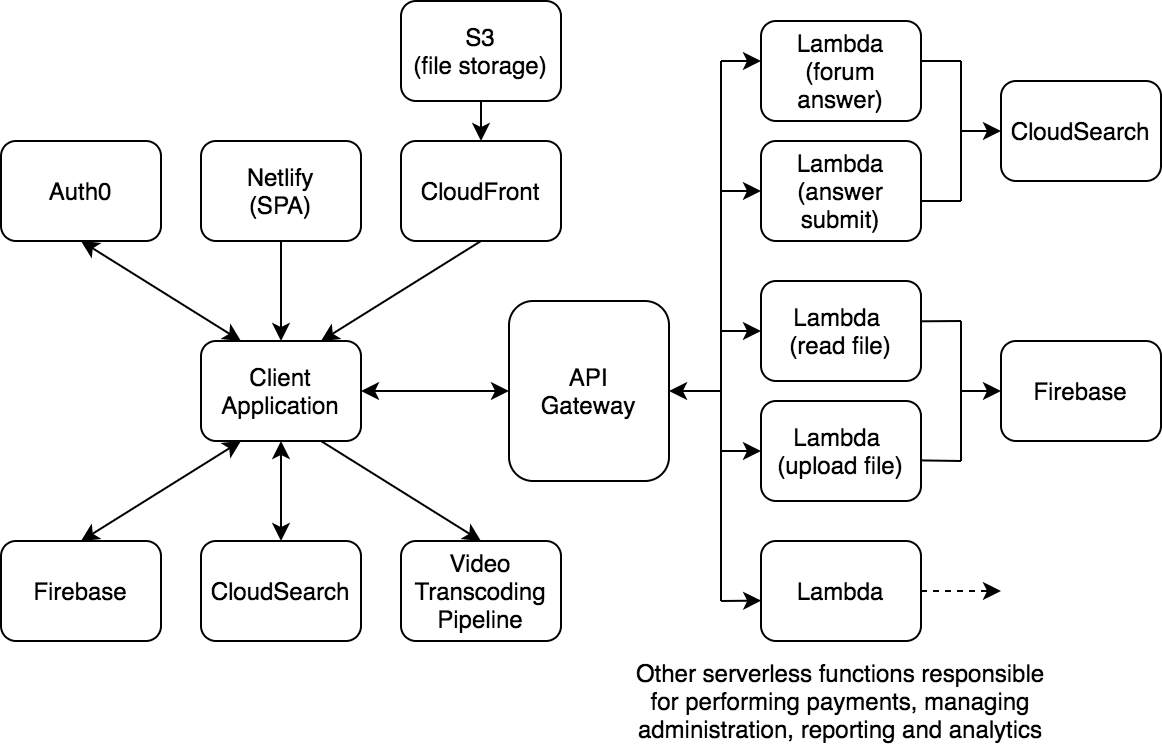
\includegraphics[width=0.8\textwidth]{assets/02-serverless/CloudGuruArchitecture.png}
    \caption{CloudGuru platform architecture}
    \label{fig:cloudguru-architecture-diagram}
\end{figure}

CloudGuru, which is an online educational platform dedicated to people interested in learning numerous cloud related topics, is a good example of such a use-case. Core features of the platform include streaming large selection of video courses, interactive quizzes and practice exams, real-time discussion forum and integrations with third party services enabling users to buy access to the courses.

The architecture of the e-learning platform utilises services of several cloud providers. Frontend of the web application built as a Single Page Application is hosted on Netlify, which acts as a Content Delivery Network (CDN) for the platform client. Auth0 service is responsible for registration and authentication functionalities and provides delegation tokens enabling client application to communicate directly and securely with other services. Firebase is used as a primary database, capable of updating clients in real-time using websockets to push updates to the clients. Questions and answers submitted by users to the forum are persisted in the Firebase, later the data is sent to AWS CloudSearch which is indexing it for further searching, enabling users to find information easier. Instructors can upload videos directly to S3 bucket, which triggers the video transcoding pipeline, which will be discussed in more details in the next section. Users can watch the videos served via CloudFront acting as a CDN if they call the lambda function beforehand giving them the permission to access the video assets for a limited period of time.

\subsection*{Event-driven data processing and manipulation}

% https://livebook.manning.com/book/serverless-architectures-on-aws/chapter-2/36 - CloudGuru

CloudGuru - transcoding videos
MindMup - exporting mindmaps

% https://livebook.manning.com/book/serverless-applications-with-node-js/chapter-15/1 -  CodePen, MindMup

\subsection*{Real-time stream processing}

\subsection*{IoT applications}

\subsection*{Webhooks / chat boots / scheduled events}

% Other articles:
% https://jyx.jyu.fi/bitstream/handle/123456789/64836/URN%3ANBN%3Afi%3Ajyu-201906253422.pdf?sequence=1
% https://www.doc.ic.ac.uk/~rbc/papers/fse-serverless-17.pdf
% https://arxiv.org/pdf/1708.08028.pdf